\documentclass[../../main.tex]{subfiles}
\begin{document}

\subsection*{7.4}
Da un selettore di velocità, che opera in un campo elettrico $E_v = 10^5\ \frac{V}{m}$ e in un campo magnetico $B_v =0.5\ T$ esce un fascio collimato di ioni $Li^+$.
\\Nel punto O, all'uscita del selettore di velocità, il fascio entra in una regione in cui esiste un campo magnetico B uniforme, parallelo al piano del disegno e formante un angolo $\theta$ con l0asse x.
\\Dopo un tempo $t = 6.28 * 10^{-6}\ s$ un aparticella si è allontanata da O di una distanza $d = 62.8\ cm$ percorrendo 10 giri attorno a B.
\\a) Calcolare la velocità degli ioni.
\\b) Calcolare il valore di B.
\\c) Calcolare il valore di $\theta$.
\\d) Calcolare il raggio r della traiettoria elicoidale.
\\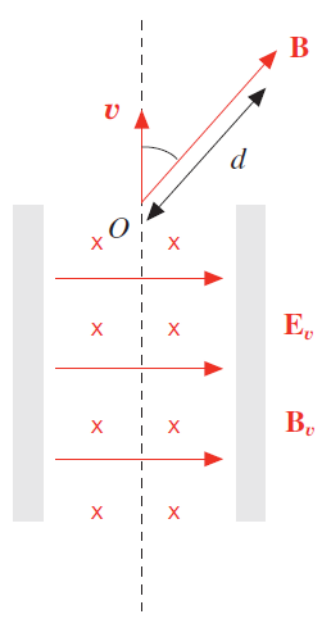
\includegraphics[scale=0.3]{e_7_4.png}
\subsubsection*{Formule utilizzate}
$\vec{F_L} = q\vec{v}\wedge\vec{B}$
\\$\vec{F_e} = q\vec{E}$
\subsubsection*{Soluzione punto a}
$\vec{F_L} + \vec{F_e} = 0$ ma se $\vec{v} \bot \vec{E}$ allora: $|\vec{F_L}| - |\vec{F_e}| = 0$
\\$vB = E$   $v= \frac{E}{B} = 2.0 * 10^5 \frac{m}{s}$
\subsubsection*{Soluzione punto b}
$\vec{F} = q\vec{v}\wedge\vec{B}$
\\$\hookrightarrow F_{\bot} = q\vec{v_{\bot}}\wedge\vec{B}$ 
\\$\hookrightarrow F_{\parallel} = q\vec{v_{\parallel}}\wedge\vec{B} = 0$
\\Se dopo 10 giri $t_10 = 6.28 * 10^{-6}\ s$
\\Un giro $t_1 = 6.28 * 19^{-7}$ 
\\$\omega = \frac{2\pi}{T}$
\\$qB = \frac{mv_\bot}{r}$
\\$B = \frac{mv_\bot}{rq}$
\subsubsection*{Soluzione punto c}
$d = v\cos\theta t$
\\$qvB = \frac{mv^2}{2}$   $qB = \frac{mv}{r}$   $r = \frac{mv}{qB}$   $r = \frac{mv\sin\theta}{qB}$
\subsubsection*{Soluzione punto d}
\newpage

\end{document}